\section{Introduction}

In the early 1930s, experiments revealed contradictions in the resistance of certain metals in the low energy regime~\cite{Meissner_1930}. In particular, the expectation at the time was that the resistance should monotonically decrease, since it is directly related to electron-phonon interactions, which decrease with decreasing temperature. However, it was found that this is not the case; in fact, the resistance of these metals reached a minimum at some temperature and then started increasing again (see Fig.~\ref{fig:classickondo} for this behavior in gold). It eventually became clear that this was due to magnetic impurities in these particular metals.

\begin{figure}[ht]
  \centering
  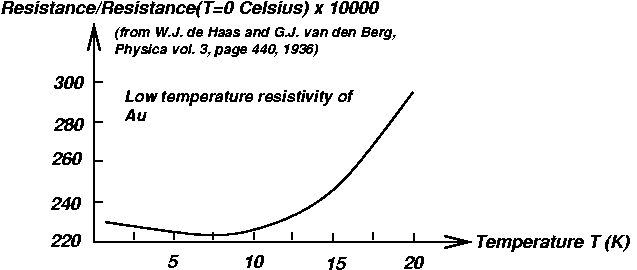
\includegraphics[width=0.6\linewidth]{../resources/gfx/classickondo.png}
  \caption{Figure created using the resistivity measurements found in \cite{DeHaas_1936}.}
  \label{fig:classickondo}
\end{figure}

At this point, a number of models were introduced in an attempt to describe a system with metallic impurities, a couple of which being the Anderson model and the s-d exchange model. These were very simple models and only account for some of the behavior observed in experiment. In 1964, one major breakthrough occurred when Jun Kondo formulated the problem as a model in which the spin of the conduction electrons interacted with that of the magnetic impurities. The Hamiltonian for this system looks like:

\begin{equation}
  \hat{H} = \sum_{\vv{k},\sigma} \epsilon_{\vv{k}}c_{\vv{k},\sigma}^\dagger c_{\vv{k},\sigma} + J\sum_{\vv{k},\vv{k}',\alpha,\beta} c_{\vv{k},\alpha}^\dagger \vv{\sigma}_{\alpha,\beta} c_{\vv{k}',\beta} \cdot \vv{S},\label{eq:kondo-hamiltonian}
\end{equation}

where $c_{\vv{k},\sigma}^\dagger$ and $c_{\vv{k},\sigma}$ are the creation and annihilation operators for Bloch states (conduction electrons) with a wavevector $\vv{k}$ and spin $\sigma$, $\epsilon_{\vv{k}}$ is the energy eigenvalue, and $\vv{S}$ is the spin of the impurity. Kondo then applied perturbation theory with this spin-spin interaction as the perturbation up to third order and retrieved results~\cite{Kondo_1964} which matched quite well with experiment; a functional form for the resistance looks like:

\begin{equation}
  R(T) = aT^5 + c_{\mathrm{imp}}R_0 - c_{\mathrm{imp}}R_1 \ln\left( \frac{k_B T}{D} \right),
\end{equation}

with the first term coming from the expected phonon interactions, the second coming from the impurities (which is temperature independent), and the third coming from perturbation theory. However, it is clear that the term logarithmic in $T$ blows up as $T \rightarrow 0$ -- it also occurs when calculating other quantities such as the entropy or specific heat. The temperature at which the resistance is most divergent is known as the \textit{Kondo temperature} $T_K$, given roughly by

\begin{equation}
  k_BT_K \approx D\exp{- \frac{1}{2J\rho}},
\end{equation}

with $D$ being the band width for the conduction electrons and $\rho$ being the density of states.

Evidently, despite accurately providing results in a particular low temperature regime, Kondo's solution wasn't perfect, and a better model was required in order to explain impurities in metals for temperatures at and below the Kondo temperature. This issue was henceforth dubbed ``The Kondo Problem''.\footnote{I am unsure if I would be honored or upset to have a rather well-known problem in physics named after my own failure to solve it...}

Soon afterwards, Philip Anderson introduced what was effectively a modifed renormalization scheme dubbed ``poor man's scaling''~\cite{Anderson_1970}. The essential recipe was a continuous scaling of the cutoff energy along with integrating out higher energy effects such that only the lower energy contributions remained, yielding an effective Hamiltonian valid at a lower energy. The reason for its peculiar name was that upon the generation of this effective Hamiltonian, the band width was not rescaled back to its original size (which would ordinarily be a step in a numerical renormalization process). It had the effect of generating further accurate solutions at low energies, but just like with the original Kondo model, the driving force was a perturbative expansion about the coupling, which upon successive renormalizations, grew to infinity. Hence, this model too become invalid at sufficiently low temperatures. Despite this, though, there was an important qualitative result: if the coupling grew without bound, then in the $T \rightarrow 0$ limit, what happens is the local moment and the conduction electrons form a bound state, called a \textit{Kondo singlet}. At this point, the observed behavior can be accounted for by virtual excitations.

Kenneth Wilson eventually took inspriation from this approach and utilized a method derived from the numerical renormalization group~\cite{Wilson_1975}, which did not involve perturbative expansion about a coupling that grew without bound, but rather about a generic small parameter $\Lambda$ related to the energy/momentum scaling factor, which remained small through the renormalization procedure. Because of this, Wilson's method was accurate at all energy scales, and finally produced coherent results for many properties at these energy scales, as well as confirming the qualitative result reached by Anderson earlier. This supported a type of \textit{asymptotic freedom}, a term first used to describe the fact that quarks become free at high energies due to the fact that the QCD coupling decreases at smaller scales.

Additionally, in 1980 and 1981, it was found by a number of independent researchers that exact solutions to Anderson's model and the s-d exchange model, could be found using the \textit{Bethe ansatz}, originally proposed by Bethe some 50 years prior in an attempt to solve the one-dimensional Heisenberg model. This was particularly noteworthy since it both confirmed the results from Wilson as well as allowing for the determination of additional thermodynamic properties and generalization to other systems.


\section{Extensions and Advancements}

Of course, with the original Kondo problem solved, physicists began looking to generalize the theory and apply it to other types of models that are more complex or adjacent in context. I give a couple such models that seem interesting.


\subsection{The Multi-Channel Kondo Model}

The original Kondo problem treated the spin of the localized magnetic moments due to the impurities as spin $1/2$ systems, and in many cases, ignored orbital angular momentum (characterized by the quantum number $\ell$), which greatly simplified calculations. One natural extension that can be made to this model is to consider spins other than $S=1/2$, or systems with multiple impurities.

This was first tackled back in the 1980's and is largely attributed to Nozi\'eres and Blandin~\cite{Nozieres_1980}, and numerous additions and corrections have been made since then; a review is given in~\cite{Schlottmann_1993}. The Hamiltonian for such a model is a straightforward modification of Eq.~\eqref{eq:kondo-hamiltonian}:

\begin{equation}
  H = \sum_{\vv{k},m,\sigma} \epsilon_{\vv{k}}c_{\vv{k},m,\sigma}^\dagger c_{\vv{k},m,\sigma} + J \sum_{\vv{k},\vv{k}',m} c_{\vv{k},m,\alpha}^\dagger \vv{\sigma}_{\alpha,\beta} c_{\vv{k}',m,\beta} \cdot \vv{S},
\end{equation}

with $m$ summing over the number of orbital channels and the sum over spins in the second term made implicit. It was found that there are three interesting regimes considering the total spin $S$ of the impurity and the number of channels $m$: when (i) $m=2S$ (\textit{perfect} screening), the number of channels can perfectly compensate the spin of the impurity, giving rise to very similar behavior to the original Kondo model and Fermi liquid behavior; when (ii) $m<2S$ (\textit{under}-screening), the the impurity spin cannot be fully compensate for the number of channels which leaves degeneracy at low temperatures and the local moment remains magnetic; and when (iii) $m<2S$ (\textit{over}-screening), the impurity spin is overcompensated for and critical behavior is observed.


\subsection{The Kondo Lattice}

The Kondo lattice is a generalization to heavy-fermion systems in which there is a lattice of impurities/local moments. Due to the translational symmetry of the lattice, the different behavior of scattered electrons gives rise to a reduction in the resistivity of these metals as opposed to the sharp incline we have seen before. The simplest Hamiltonian for the Kondo lattice looks like:

\begin{equation}
  H = \sum_{\vv{k},\sigma} \epsilon_{\vv{k}}c_{\vv{k},\sigma}^\dagger c_{\vv{k},\sigma} + J \sum_j c_{j,\alpha}^\dagger \vv{\sigma}_{\alpha,\beta} c_{j,\beta} \cdot \vv{S}_j,
\end{equation}

where

\begin{equation}
  c_{j,\sigma}^\dagger = \frac{1}{\sqrt{N_s}} \sum_{\vv{k}} c_{\vv{k},\sigma}^\dagger e^{-i\vv{k}\cdot\vv{R}_j}
\end{equation}

is the creation operator for an electron at cite $J$ and normalized to the number of states.

This is a very rich model with lots of underlying physics, some of which has yet to be fully ironed out today, and as such, even the basics are very confusing to me at this stage, so I will leave it at this basic description.


\section{Project Objectives}

Some objectives for this project is to delve deeply into the numerical renormalization group solution proposed by Wilson and its applicability to the Kondo problem, along with understanding the Anderson impurity and s-d exchange models and their exact solutions via the Bethe ansatz. From here, I will plan to explore some of the generalizations of these models and their solutions to some other problems, such as the multi-channel Kondo model and the Kondo lattice. Though, as mentioned in the previous section, since the Kondo lattice is still an area of active research today, it would be a monumental task to try understand all of it, so I will do my best to explore only some of the basics of what has currently been done.

Also, due to the nice iterative nature of Wilson's perturbative numerical renormalization technique, it is particularly well suited for computational analysis. Since I am very actively programming for my current research, I think that attempting to implement the technique and comfirming some of the results on my own would be benefical and super interesting. Further, renormalization is something I have briefly studied before in high-energy physics, so seeing it in a new context would be very helpful for my future studies/research. Due to these things, the main component of this project will be on the renormalization solution(s) to the Kondo problem. As a tentative final goalpost, I would like to accurately and confidently reproduce some of the thermodynamic quantities Wilson originally calculated via my own program implementation.

To continue with this point, I know we touched on this a little while back before I was fully set on the Kondo problem, but I am unsure where, let alone how, I would be able to find an unexplored corner of this model. It seems very well researched, and any such corners would be mighty challenging to solve, especially for a high-energy physicist. If there are any such small corners that are feasible, it would be good to know, but there is such a wealth of information it is very hard to find anything myself.

\subsection{Resources}

There are quite a number of resources covering this topic. One of the main source I plan to use is the book ``The Kondo problem to heavy fermions'' by Alexander Cyril Hewson~\cite{Hewson_1993}, which contains a ton of information related to all of the aforementioned concepts and is used as a reference by a number of other sources I've found. Unfortunately, Hewson himself states the book is intended for second and third year post-graduate students, so the content may be quite challenging to digest. Despite this, it will be immensely helpful for this project, and I've already started reading a bit into it.

Another good resource I have found are the lecture notes from a summer school in Germany related to many body physics, in particular the Kondo problem/effect and related topics~\cite{manybodyphys_2015}. There were 15 independent lectures, most of them are likely not going to be entirely applicable to this project, but a handful will be, namely the first 5 or so. They are essentially a crash course in some of the topics I've just discussed, leaving some of the specifics out but providing a good overview. Importantly, they also contain a plethora of references which I can explore should I need more information about a particular topic, some of which I've already cited in this report.

Lastly, the original papers of the physicists who made these advancements (many of which I have already directly cited when introducing the major results) will be useful, even if I can only gleam the basic ideas from them, as they will no doubt be packed with things I cannot hope to understand.

\subsection{Physical Materials}

Lastly, as it was implied in the email you sent a couple weeks back (before break) with the basic requirements for this proposal, I will also comment on the fact that this project won't require any physical materials. All work would be done on paper and computer.




%%% Local Variables:
%%% mode: LaTeX
%%% TeX-master: "../project"
%%% End:
